\newpage

\section{Methodology of the Survey}
\label{app:methodology}

\subsection{Search Strategy}
\label{app:search-strategy}

Because agent context compression is an emerging topic without a unified terminology, we adopted a broad search strategy rather than relying on a single keyword. We searched ACL Anthology, DBLP, arXiv, Google Scholar, Semantic Scholar, and major NLP, machine learning, software engineering, and agent-system venues. The search covered both explicit compression terms and adjacent terms used in related communities.

Specifically, we used keyword combinations such as \textit{``LLM agent''} with \textit{``context compression''}, \textit{``trajectory compression''}, \textit{``history summarization''}, \textit{``context pruning''}, \textit{``context folding''}, \textit{``agent memory compression''}, \textit{``memory retrieval''}, and \textit{``long-horizon agent context''}. We also searched domain-specific terms, including \textit{``coding agent context''}, \textit{``web agent memory''}, \textit{``GUI agent observation compression''}, and \textit{``deep research agent memory''}. These queries were designed to capture papers that may not use the exact phrase \textit{context compression} but nevertheless reduce, rewrite, externalize, or retrieve agent history under a limited context budget.

In addition to keyword search, we performed backward and forward citation tracing from representative work on prompt compression, long-context modeling, agent memory, web agents, coding agents, and deep-research agents. This step was necessary because many relevant systems describe compression-related operations as \textit{memory management}, \textit{state retention}, \textit{context engineering}, \textit{trajectory summarization}, or \textit{retrieval-based continuation}. We therefore treated terminology flexibly and focused on whether a method changes what historical information remains available to the agent during future execution.

\subsection{Inclusion and Exclusion Criteria}
\label{app:inclusion-exclusion}

We included a paper or system if it satisfied at least one of the following conditions. First, it proposes a method that compresses, filters, summarizes, prunes, folds, externalizes, or retrieves the context of an LLM agent during multi-step execution. Second, it introduces a memory or retrieval mechanism whose purpose is to preserve task-relevant information under a finite context budget. Third, it analyzes long-horizon agent behavior in a way that reveals failures caused by context reduction, memory selection, retrieval, or compressed-state reuse. Fourth, it describes a deployed or production-grade agent system with publicly documented context-management behavior relevant to the operational pipeline studied in this survey.

We excluded work whose primary contribution lies outside application-level agent context management. In particular, we excluded methods that only compress static, single-turn prompts unless they are explicitly adapted to multi-step agent trajectories. We also excluded model-level compression methods, such as weight quantization, model pruning, distillation, and generic KV-cache optimization, when they do not alter the information available to the agent as part of its executable context. Similarly, general retrieval-augmented generation was not treated as agent context compression unless retrieval is coupled to an evolving agent state, trajectory history, or memory store.

For borderline cases, we used a functional criterion: a work was considered relevant if its method changes how past observations, actions, thoughts, plans, or memory states are preserved and reused for future decisions under a context constraint. This criterion allowed us to include systems that do not explicitly use the term \textit{compression} but still perform compression-like state management. When a method combined multiple components, such as summarization plus retrieval or pruning plus external memory, we categorized it according to the component that most directly determines the compressed state available to later agent execution.

Finally, for production-grade systems and technical reports, we only relied on public evidence and high-confidence descriptions. When implementation details were unavailable, we characterized the system at the level of observable pipeline behavior rather than making assumptions about proprietary mechanisms.


\section{Extended Taxonomies and Resources}
\label{ap:extended_taxonomies}

\subsection{Details about taxonomy}
\label{ap:details_about_taxonomy}
In the main text, we characterize context management methodologies based on three core dimensions, specifically \textit{when}, \textit{what}, and \textit{how}, while further analyzing their application \textit{domain} as a complementary perspective. Table~\ref{tab:full_taxonomy} below instantiates this framework at the level of individual methods. Specifically, the \textit{when} column indicates the trigger mechanism and decision maker for context compression or management, including system-controlled, external-controller, agent-controlled, and learned policies; the \textit{what} column identifies the context object being managed, such as observations, trajectories, memory states, plans and reasoning traces, or representation-level signals; and the \textit{how} column summarizes the compression mechanism, including truncation and masking, pruning and reduction, summarization and abstraction, externalization and retrieval, and representation-level compression. In addition to these three dimensions, we report the \textit{domain} of each method to indicate its primary task setting, and we analyze its distribution and characteristics separately in the main text. Taken together, the table provides a fine-grained view of how different methods are positioned within the taxonomy and how their design choices vary across task domains.

\subsection{Open-Source Standouts}
\label{ap:open_source_standouts}
To more comprehensively reflect the openness and reproducibility of research in this area, we further collected and summarized the open-source methods included in this survey, as shown in Table~\ref{tab:opensource_methods}. The table exclusively incorporates methods accompanied by publicly available code, presenting them across three columns: method name, open-source link, and publication year. This organization enables readers to efficiently locate the corresponding implementations and repository resources. As shown in the table, the current open-source work is concentrated in a small number of representative methods, and the release years span 2025 to 2026, which indicates that this field is still evolving rapidly and that its open-source ecosystem is steadily maturing. Overall, this statistics not only improves the reproducibility of our survey results, but also provides a direct entry point for future researchers to conduct method comparison, code replication, and further development.

\subsection{Datasets \& Benchmarks}
Table~\ref{tab:datasets_benchmarks} summarizes the representative datasets and benchmarks collected in \texttt{datasets\_info.md}. We organize them by task family and retain only the information most useful for a survey on agentic context management: benchmark purpose, publication venue/year, and public availability. To keep the table compact, we move the task-focus and scale description into the benchmark cell itself, so each row reads as a short self-contained summary.

The \emph{Benchmark} cell includes the dataset name, a citation to the original paper, and a brief description of the task and scale. The \emph{Source and year} column records the original publication venue or release year, while the \emph{Open Source} column provides the public repository or dataset URL when available, and indicates the absence of public releases otherwise. Benchmarks with closely related variants are grouped together to keep the presentation compact.

First, the selected benchmarks are intentionally diverse, encompassing software engineering, web browsing, office automation, mobile apps, deep research, long-context reasoning, memory, code generation, and long-document summarization. This diversity is essential, as context management methods frequently navigate the trade-off between retaining essential task-critical evidence and pruning redundant historical data, with individual benchmarks typically evaluating only a specific subset of these behaviors.

Second, numerous benchmarks are structured as closely related families or variants. For instance, \emph{SWE-bench Verified}~\citep{jimenez2024swebench} and \emph{SWE-bench Lite}~\citep{jimenez2024swebench} assess software issue resolution under different difficulty and edit constraints; \emph{BrowseComp}~\citep{wei2025browsecomp}, \emph{BrowseComp-Plus}~\citep{chen2025browsecompplus}, and \emph{BrowseComp-ZH}~\citep{zhou2025browsecompzh} cover browsing-centric deep search in different settings; \emph{Mind2Web}~\citep{deng2023mind2web} and \emph{Multimodal-Mind2Web}~\citep{zheng2024seeact} differ by adding visual grounding; \emph{LongBench}~\citep{bai2024longbench}, \emph{LongBench V2}~\citep{bai2025longbenchv2}, \emph{BABILong}~\citep{NEURIPS2024_babilong}, \emph{NeedleBench}~\citep{li2024needlebench}, and \emph{NIAH}~\citep{liu2023lost} probe long-context handling from complementary angles.

Third, in instances where a benchmark entry represents a comprehensive framework or family rather than an isolated dataset, we designate it by its representative name in the table and elucidate the included variants within the accompanying notes. This is especially helpful for benchmarks such as \emph{MRQA}~\citep{fisch-etal-2019-mrqa}, \emph{Loghub}~\citep{zhu2023loghub}, and \emph{CompileBench / CRUST-Bench}~\citep{khatry2025crustbench}, where a single umbrella name aggregates multiple sub-datasets or tasks.

Finally, the \emph{Open Source} column is interpreted broadly, providing the public dataset or repository URL when available, and explicitly noting cases where no public release could be identified within the collected sources. The original publication year and venue are preserved in the \emph{Source and year} column.


\section{Implementation Details of Compression Operators}
\label{app:operator-details}

This appendix supplements the taxonomy in Section~\ref{subsec:compression_mechanism} by summarizing concrete implementation details of representative compression operators. We focus on three methods with relatively explicit descriptions: ReSum \citep{wu2026resumunlockinglonghorizonsearch} and AgentFold  \citep{ye2025agentfoldlonghorizonwebagents} for summarization and abstraction, and SWE-Pruner \citep{wang2026sweprunerselfadaptivecontextpruning} for pruning and reduction. The goal is not to reproduce full prompts verbatim, but to identify the prompt roles, response templates, algorithmic steps, and compression-specific design choices that instantiate the operator families discussed in the main text.

\subsection{Prompts for Summarization and Abstraction}
\label{app:prompts-summarization}

Summarization and abstraction methods rewrite long interaction histories into shorter executable states. Table~\ref{tab:app-c1-prompts} compares the concrete prompt or response-template designs in ReSum and AgentFold. ReSum exposes summarization as a separate tool invocation that periodically converts a growing trajectory into a compact restartable state. AgentFold, by contrast, embeds context folding into the agent's own structured response format, so that the agent jointly reasons, updates its compressed state, and acts.

\begin{table*}[t]
\centering
\small
\setlength{\tabcolsep}{3pt}
\renewcommand{\arraystretch}{1.08}

\begin{tabularx}{\textwidth}{@{}
>{\raggedright\arraybackslash}p{1.55cm}
>{\raggedright\arraybackslash}p{2.25cm}
>{\raggedright\arraybackslash}X
>{\raggedright\arraybackslash}X
>{\raggedright\arraybackslash}X
@{}}
\hline
\textbf{Method} & \textbf{Prompt / Template} & \textbf{Input} & \textbf{Output} & \textbf{Compression-specific instruction} \\
\hline
ReSum \citep{wu2026resumunlockinglonghorizonsearch}
&
Context summarization prompt
&
The original question and the accumulated conversation history, which may include the agent's previous reasoning, tool calls, observations, and intermediate findings.
&
A compact summary block that condenses the previous trajectory into a restartable reasoning state.
&
The summary tool is instructed to extract task-relevant and reliable information from the history, preserve useful evidence and search progress, and avoid unsupported guesses or uncertain inferences.
\\
\hline
ReSum \citep{wu2026resumunlockinglonghorizonsearch}
&
Summary-conditioned reasoning prompt
&
The original question together with the generated summary from previous exploration.
&
Continued reasoning and tool use conditioned on the generated summary.
&
The agent is instructed to treat the summary as condensed prior context, judge whether it is sufficient, and continue collecting evidence if the summary does not yet support a final answer.
\\
\hline
AgentFold \citep{ye2025agentfoldlonghorizonwebagents}
&
Structured agent response template
&
The task instruction, tool interface, current multi-scale state summaries, and latest high-fidelity interaction.
&
A structured response containing thinking, a folding directive, a brief explanation, and the next tool call/action.
&
Context management is made part of the agent's action space. Each step can update the compressed state while still preserving the latest interaction at high fidelity for immediate reasoning.
\\
\hline
AgentFold \citep{ye2025agentfoldlonghorizonwebagents}
&
Folding directive template
&
Existing state summaries plus the latest interaction.
&
A JSON-like folding command specifying which span should be folded and what summary should replace it.
&
The directive supports two modes: granular condensation, which folds a single latest step while preserving useful information, and deep consolidation, which folds several steps into a coarser summary when they complete a subtask and their intermediate details are no longer critical for further task solving.
\\
\hline
\end{tabularx}
\caption{Prompt and response-template details for summarization and abstraction methods. ReSum uses explicit summarization and summary-conditioned reasoning prompts, whereas AgentFold embeds context folding into the agent's structured response format.}
\label{tab:app-c1-prompts}
\end{table*}

Table~\ref{tab:app-c1-flow} further summarizes the operational flow of the two methods. Although both methods compress trajectories through natural-language abstraction, their control policies differ. ReSum is closer to periodic tool-mediated summarization, while AgentFold is closer to agent-controlled online state maintenance.

\begin{table*}[t]
\centering
\small
\setlength{\tabcolsep}{3pt}
\renewcommand{\arraystretch}{1.08}

\begin{tabularx}{\textwidth}{@{}
>{\raggedright\arraybackslash}p{1.55cm}
>{\raggedright\arraybackslash}p{1.85cm}
>{\raggedright\arraybackslash}X
>{\raggedright\arraybackslash}X
>{\raggedright\arraybackslash}X
@{}}
\hline
\textbf{Method} & \textbf{Trigger} & \textbf{Compression process} & \textbf{Resulting state} & \textbf{Main risk} \\
\hline
ReSum \citep{wu2026resumunlockinglonghorizonsearch}
&
Periodic or budget-driven summarization during long-horizon search.
&
The agent accumulates a ReAct-style trajectory until summarization is invoked. The summarizer rewrites the prior history into a compact state, after which the agent continues from the original question plus the generated summary rather than the full history.
&
A compact, restartable reasoning state that retains prior discoveries, useful clues, and unresolved directions.
&
The summary may omit evidence, over-compress uncertainty, or fail to preserve fine-grained dependencies needed in later search.
\\
\hline
AgentFold \citep{ye2025agentfoldlonghorizonwebagents}
&
Agent-initiated folding at each step.
&
At each step, the agent keeps the most recent interaction as high-fidelity working memory and issues a folding directive that either condenses a single step into a fine-grained summary or consolidates multiple steps into a coarser summary.
&
A multi-scale memory state consisting of fine-grained local summaries and coarser strategic summaries.
&
The agent may fold too aggressively, consolidate heterogeneous intermediate steps, or abstract away details that later become necessary.
\\
\hline
\end{tabularx}
\caption{Operational flow of ReSum and AgentFold. Both compress trajectories into executable summaries, but they differ in whether summarization is invoked as an external tool or internalized as an agent action.}
\label{tab:app-c1-flow}
\end{table*}

\subsection{Algorithms for Pruning and Reduction}
\label{app:algorithms-pruning}

Pruning and reduction methods differ from abstractive summarization because they preserve selected source content exactly. This property is especially important for coding agents, where identifiers, file paths, syntax, and local dependencies often need exact retention. SWE-Pruner \citep{wang2026sweprunerselfadaptivecontextpruning} is a representative pruning-based method: it operates as a middleware between the coding agent and the environment, intercepts long code observations, and returns a shorter pruned observation to the agent.


The core scoring and aggregation procedure can be summarized as Algorithm~\ref{alg:swe-pruner}. The notation is simplified to emphasize the compression operator rather than implementation-specific training details.

\begin{algorithm}[t]
\small
\caption{Task-aware line-level pruning in SWE-Pruner}
\label{alg:swe-pruner}
\begin{algorithmic}[1]
\REQUIRE Code context $C$, pruning query or goal hint $q$, scoring model $F_{\theta}$, threshold $\tau$
\ENSURE Pruned code context $\tilde{C}$
\STATE Split $C$ into lines $L=\{l_1,\ldots,l_m\}$
\STATE Tokenize $C$ into tokens $X=\{x_1,\ldots,x_n\}$
\FOR{each token $x_i \in X$}
    \STATE Compute token relevance score $s_i = F_{\theta}(x_i, C, q)$
\ENDFOR
\FOR{each line $l_j \in L$}
    \STATE Let $T_j$ be the set of tokens belonging to line $l_j$
    \STATE Aggregate token scores into a line score:
    \[
    \bar{s}_j = \frac{1}{|T_j|}\sum_{x_i \in T_j} s_i
    \]
\ENDFOR
\STATE Decode or threshold line scores to obtain keep/drop labels $y_j \in \{0,1\}$
\STATE Construct $\tilde{C}$ by preserving lines with $y_j=1$
\RETURN $\tilde{C}$
\end{algorithmic}
\end{algorithm}


\section{Case Studies of Context Compression Failure Modes}
\label{app:case-studies-compression-failures}

This appendix provides three illustrative cases corresponding to the temporal failure taxonomy in Section~\ref{sec:4_failure_modes}. 
Each case follows the same pipeline: a task produces an original agent trajectory; the trajectory is compressed into a compact state; and the downstream agent fails after compression. 
The cases are constructed to clarify where the earliest causal error arises in the compression pipeline: before compression, during compression, or after compression.

% \begin{figure*}[t]
%     \centering
%     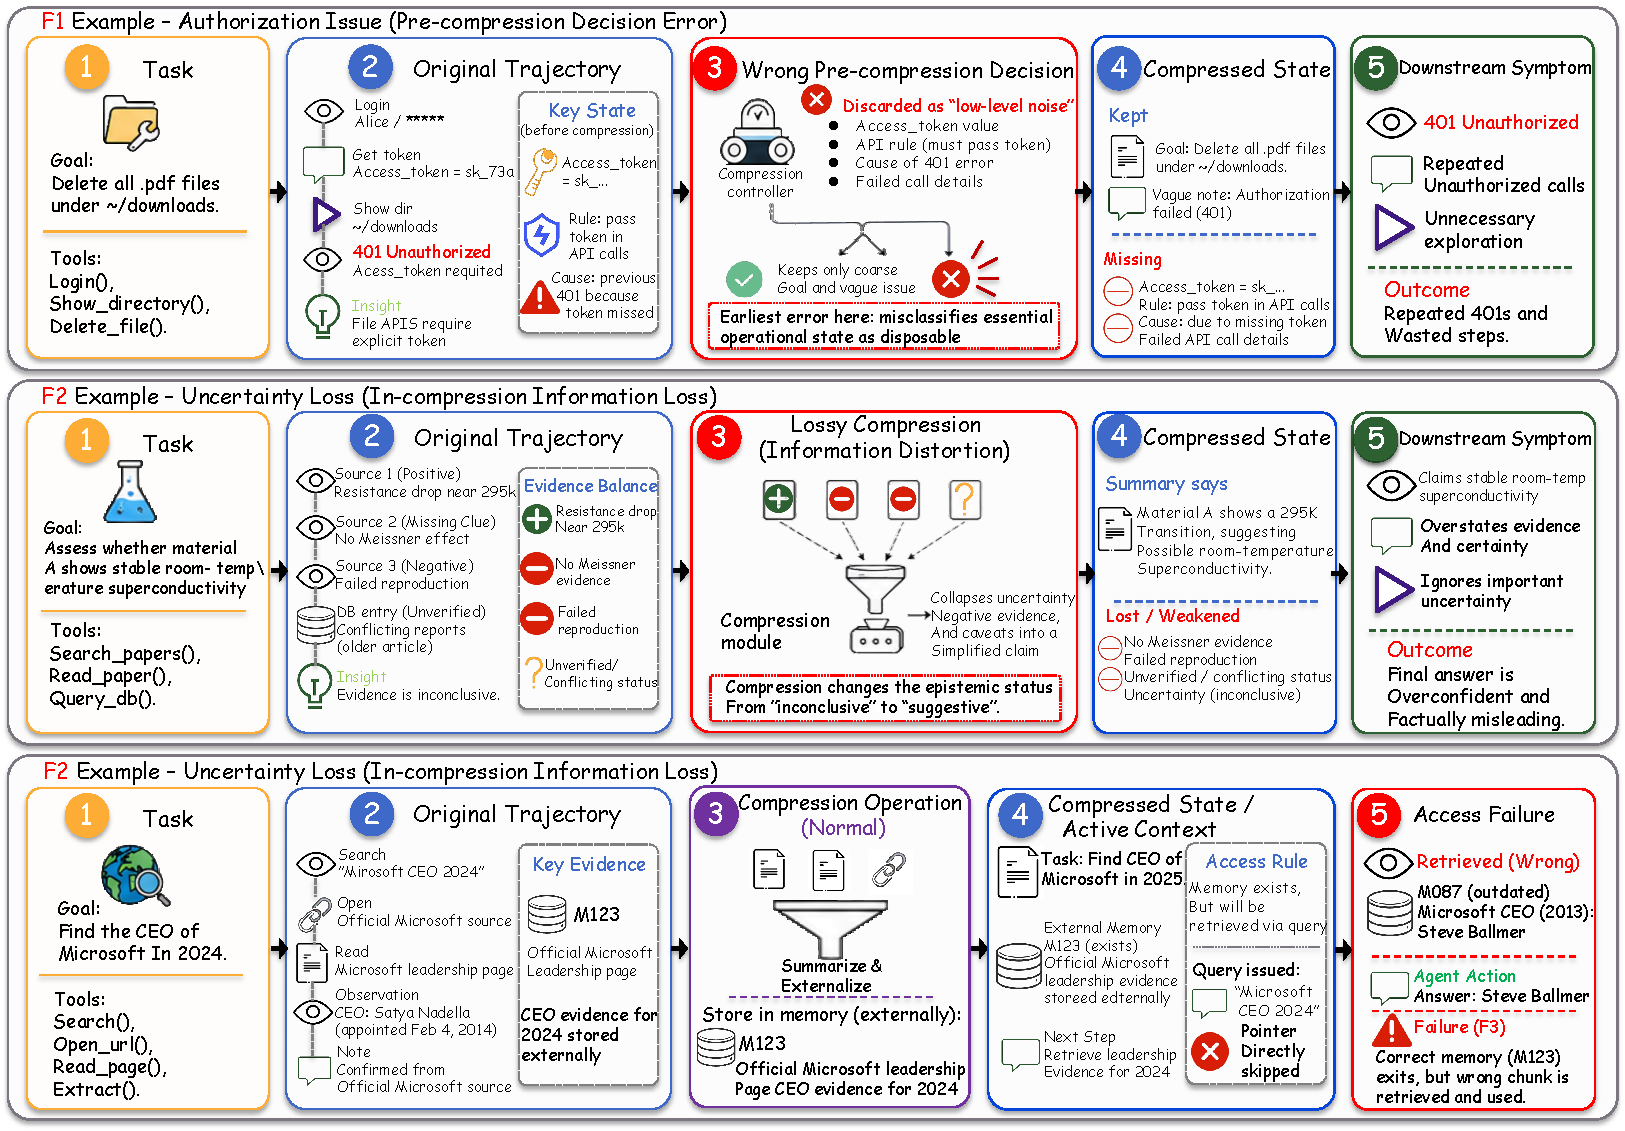
\includegraphics[width=\textwidth]{figures/cases123.pdf}
%     \caption{
%     Three illustrative cases of context compression failure modes. 
%     F1 shows a pre-compression decision error, where the compression controller misclassifies authentication state and API-call details as low-level noise before summarization. 
%     F2 shows in-compression information loss, where a compression module distorts the evidential balance by weakening uncertainty, negative evidence, and caveats. 
%     F3 shows a post-compression access failure, where the correct memory item exists after compression but is not correctly expanded or retrieved, causing the agent to use an outdated wrong chunk.
%     }
%     \label{fig:case-studies-compression-failures}
% \end{figure*}

\subsection{F1 Example -- Authorization State Dropped}
\label{app:case-f1-auth-state}

Figure~\ref{fig:case-studies-compression-failures}a illustrates an F1 failure in a file-management task. 
The agent is asked to delete all \texttt{.pdf} files under \texttt{\textasciitilde/downloads}. 
In the original trajectory, the agent logs in, obtains an \texttt{access\_token}, attempts to inspect the target directory, and observes a \texttt{401 Unauthorized} response. 
The failed API call is not merely an incidental error: it reveals an operational rule that every subsequent file-system API call must explicitly pass the access token.

The crucial state before compression therefore consists of three linked pieces of information: the concrete token value, the API rule requiring the token, and the cause of the previous \texttt{401} error. 
However, the compression controller makes a wrong pre-compression retention decision. 
It treats the token, the failed API-call details, and the token-passing rule as disposable low-level execution noise, while preserving only the coarse task objective and a vague note that authorization failed.

The resulting compressed state is insufficient for correct continuation. 
After compression, the downstream agent still knows that it should delete PDFs under the target directory, but it no longer knows how to perform authorized API calls. 
It therefore repeats unauthorized calls and wastes steps on unnecessary exploration.

This is an F1 failure because the earliest causal error occurs before the compression operation itself. 
The problem is not that the summarizer distorted selected content, nor that a saved memory could not be retrieved later. 
Rather, the controller incorrectly decided that essential operational state was not worth preserving. 
The repeated \texttt{401} errors are downstream symptoms of this pre-compression decision error.

\subsection{F2 Example -- Uncertainty Loss}
\label{app:case-f2-uncertainty-loss}

Figure~\ref{fig:case-studies-compression-failures}b illustrates an F2 failure in a research-agent task. 
The agent is asked to assess whether Material A shows stable room-temperature superconductivity. 
The original trajectory contains heterogeneous evidence: one source reports a resistance drop near 295K, another reports no Meissner evidence, a third source reports failed reproduction, and a database entry marks the claim as unverified with conflicting reports. 
The agent's intermediate conclusion is therefore cautious: the evidence is inconclusive.

Unlike the F1 case, the relevant evidence has been collected and is available to the compression module. 
The failure occurs during compression. 
When the trajectory is condensed, the compression module collapses the evidence balance into a simplified statement that Material A shows a 295K transition, suggesting possible room-temperature superconductivity. 
At the same time, the negative and uncertainty-bearing evidence is weakened or dropped: the lack of Meissner evidence, failed reproduction, unverified database status, and overall inconclusiveness no longer strongly constrain the compressed state.

This is an F2 failure because the compression process changes the epistemic status of the trajectory. 
The original evidence supports an inconclusive assessment, but the compressed state makes the claim appear more suggestive and better supported than it actually is. 
The downstream agent then overstates the evidence and produces an overconfident, factually misleading final answer.

The key distinction from F1 is that the information was not excluded by a prior retention decision. 
Instead, the evidence entered the compression step but was transformed into a less faithful representation. 
Thus, the earliest causal error lies inside the compression operation itself.

\subsection{F3 Example -- Wrong Retrieval}
\label{app:case-f3-wrong-retrieval}

Figure~\ref{fig:case-studies-compression-failures}c illustrates an F3 failure in a web-research task. 
The agent must find the CEO of Microsoft in 2024. 
In the original trajectory, it searches for ``Microsoft CEO 2024'', opens an official Microsoft source, reads the leadership page, and observes that Satya Nadella was appointed Chief Executive Officer of Microsoft on February 4, 2014. 
This correct evidence is then summarized and externalized as memory item \texttt{M123}, which stores the official Microsoft leadership evidence for the 2024 CEO.

Unlike the F2 case, the relevant information is not lost or distorted during compression. 
The compression operation successfully externalizes the correct evidence. 
However, the compressed active context does not contain the full content of \texttt{M123}; it contains the task, an external memory pointer, and an access mechanism indicating that the evidence should be retrieved when needed. 
The correct memory therefore exists, but it must re-enter the active context through a post-compression access step.

The failure occurs after compression. 
Instead of directly expanding the correct pointer \texttt{M123}, the agent issues the query ``Microsoft CEO 2024''. 
The retrieval mechanism returns a different memory item, \texttt{M087}, which is topically related but temporally mismatched: it states that Steve Ballmer was Microsoft CEO in 2013 based on an older article. 
The downstream agent integrates this wrong retrieved chunk into the active context and answers Steve Ballmer.

This is an F3 failure because the correct information has been retained, but it is not correctly accessed at the decision point. 
The earliest causal error is neither a pre-compression decision error nor an in-compression distortion. 
Rather, it is a post-compression access failure: the correct memory item \texttt{M123} exists, but the retrieval or expansion mechanism surfaces \texttt{M087} instead. 
The final answer is wrong because the agent reasons from the wrong retrieved memory, not because the correct evidence was never stored.


\section{Extended Future Directions}
\label{ap:extended_future_directions}

\paragraph{The Compression--Retrieval--Memory Boundary}
In current agent systems, compression, retrieval, and external memory are often combined, but they serve different functions and have different recoverability properties. A more principled framework is needed to determine when information should be compressed, when it should be stored externally, and when it should remain in active context.


\paragraph{Learning to Compress Recoverably}
Most existing learned policies optimize task success and token efficiency, but these objectives do not directly capture whether compressed information can be reconstructed when needed. Future work should incorporate recoverability and dependency preservation into both training objectives and evaluation.

\paragraph{Compression in Multi-Agent Systems}
When context is shared across agents, compression becomes a communication and coordination problem rather than a local memory optimization problem. This setting raises new questions about what should be summarized, what should be shared verbatim, and how compression errors propagate across agents.

\paragraph{End-to-End Training under Context Budgets}
Compression is usually treated as a separate module from planning and tool use, even though these decisions are tightly coupled in long-horizon agents. Joint optimization under explicit budget constraints may better align compression behavior with downstream task performance.

\paragraph{Domain-Specific Compression Methods}
As shown in \S~\ref{sec:5_domain_specific_analysis}, coding, web/GUI, and research agents impose different requirements on structural fidelity, recoverability, and evidence precision. This suggests that domain-tailored compression strategies will be important in addition to general-purpose methods.

\paragraph{Standardized Benchmarks and Reproducibility}
Existing work differs widely in agent backbone, task set, budget, and compressed target, which makes direct comparison difficult. Future benchmarks should report not only task success and token savings, but also information density, recoverability, error propagation, and controller overhead under controlled settings.

\paragraph{Concluding Discussion}

Agent context compression is no longer just a preprocessing convenience. For long-horizon agents, it is a state-management problem over a changing workspace, not a one-shot prompt-shortening step. This survey structures the area along three axes: targets, mechanisms, and control policies. It also introduces a failure taxonomy and an evaluation framework that goes beyond task success. The key challenge is not only stronger compression, but compression that remains recoverable, faithful, and aligned with long-term agent execution.


\newcommand{\coding}[1][1.1em]{
\includegraphics[width=#1]{icons/coding.pdf}}
\newcommand{\web}[1][1.3em]{
\includegraphics[width=#1]{icons/web.pdf}}
\newcommand{\search}[1][1.2em]{
\includegraphics[width=#1]{icons/search.pdf}}
\newcommand{\gui}[1][1.2em]{
\includegraphics[width=#1]{icons/gui.pdf}}
\newcommand{\research}[1][1.2em]{
\includegraphics[width=#1]{icons/research.pdf}}
\newcommand{\general}[1][1.2em]{
\includegraphics[width=#1]{icons/general.pdf}}

\captionsetup[longtable]{belowskip=0.5em}  % 调整这个值，正值增加距离

% Table 2 (EMNLP style, auto page-break + auto line-wrap version)
% This file is self-contained for two-column papers:
% temporarily switch to one-column so longtable can work, then switch back.

\clearpage
\onecolumn

\footnotesize
\setlength{\tabcolsep}{2pt}
\renewcommand{\arraystretch}{1.06}

% Force wrapping behavior in every cell (including long tokens / URLs-like strings).
\sloppy

% Keep total width within one-column text width to avoid overfull hboxes.
\begin{longtable}{>{\raggedright\arraybackslash\hspace{0pt}}p{0.5cm} >{\raggedright\arraybackslash\hspace{0pt}}p{2.25cm} >{\raggedright\arraybackslash\hspace{0pt}}p{2.4cm} >{\raggedright\arraybackslash\hspace{0pt}}p{2.50cm} >{\raggedright\arraybackslash\hspace{0pt}}p{2.50cm} >{\raggedright\arraybackslash\hspace{0pt}}p{2.50cm} >{\raggedright\arraybackslash\hspace{0pt}}p{1.50cm}}

\toprule[1.5pt]
\textbf{ID} & \textbf{Method} & \textbf{Author \& Year} & \textbf{When} & \textbf{What} & \textbf{How} & \textbf{Domain} \\
\hline
\endfirsthead

\multicolumn{7}{r}{\footnotesize Continued from previous page} \\
\toprule[1.5pt]
\textbf{ID} & \textbf{Method} & \textbf{Author} & \textbf{When} & \textbf{What} & \textbf{How} & \textbf{Domain} \\
\hline
\endhead

\hline
\multicolumn{7}{r}{\footnotesize Continued on next page} \\
\endfoot

\bottomrule[1.5pt]

\caption{Full Taxonomy Coordinates. Domain icons: \coding[0.85em]~Coding Agents, \web[0.85em]~Web Agents, \gui[0.85em]~GUI Interaction Agents, \search[0.85em]~Deep-Search Agents, \research[0.85em]~Research Agents, \general[0.85em]~General Agents.}
\label{tab:full_taxonomy} \\
\endlastfoot


1 & WebAgent & \citealp{gur2024realworldwebagentplanninglong} & System-Controlled & Observation & Summarization \& Abstraction & \web \gui \\
2 & PAL-UI & \citealp{liu2025paluiplanningactivelookback} & Agent-Controlled & Trajectory & Externalization \& Retrieval & \web \gui \\
3 & LCoW & \citealp{lee2025learningcontextualizewebpages} & Learned & Observation & Summarization \& Abstraction & \web \gui \\
4 & Sculptor & \citealp{li2025sculptorempoweringllmscognitive} & Agent-Controlled & Memory State & Truncation \& Masking / Abstraction & \general \\
5 & SWE-Pruner & \citealp{wang2026sweprunerselfadaptivecontextpruning} & Learned & Observation & Pruning \& Reduction & \coding \\
6 & AgentOCR & \citealp{feng2026agentocrreimaginingagenthistory} & Agent-Controlled & Trajectory & Representation-Level & \search \research \\
7 & Step-DeepResearch & \citealp{hu2025stepdeepresearchtechnicalreport} & System-Controlled & Observation & Externalization \& Retrieval & \search \research \\
8 & MCP-Bench & \citealp{wang2025mcpbenchbenchmarkingtoolusingllm} & System-Controlled & Observation & Summarization \& Abstraction & \general \\
9 & PAACE & \citealp{yuksel2025paaceplanawareautomatedagent} & Learned & Plan \& Reasoning & Pruning / Abstraction & \general \\
10 & WebWeaver & \citealp{li2025webweaverstructuringwebscaleevidence} & Agent-Controlled & Memory State & Externalization \& Retrieval & \search \research \\
11 & The Complexity Trap & \citealp{lindenbauer2025complexitytrapsimpleobservation} & System-Controlled & Observation & Truncation \& Masking & \coding \\
12 & WebClipper & \citealp{wang2026webclipperefficientevolutionweb} & Learned & Trajectory & Pruning \& Reduction & \search \research \\
13 & AOI & \citealp{bai2026aoicontextawaremultiagentoperations} & System-Controlled & Memory State & Summarization \& Abstraction & \coding \\
14 & COMPASS & \citealp{wan2025compassenhancingagentlonghorizon} & External Controller & Plan \& Reasoning & Summarization \& Abstraction & \search \research \\
15 & ACC & \citealp{bousetouane2026aiagentsneedmemory} & External Controller & Memory State & Summarization \& Abstraction & \general \\
16 & BACM & \citealp{xiao2025improving} & Agent-Controlled & Trajectory & Summarization \& Abstraction & \search \research \\
17 & Q-KVComm & \citealp{kriuk2025qkvcommefficientmultiagentcommunication} & System-Controlled & Representation-Level & Representation-Level & \general \\
18 & Visual MAD & \citealp{wu2026crossmodalmemorycompressionefficient} & System-Controlled & Trajectory & Representation-Level & \general \\
19 & SCMA & \citealp{chen2026selfcompressionchainofthoughtmultiagentreinforcement} & Learned & Plan \& Reasoning & Pruning \& Reduction & \general \\
20 & CSIM & \citealp{liu2025csim} & Learned & Plan \& Reasoning & Summarization \& Abstraction & \search \research \\
21 & ACON & \citealp{kang2025aconoptimizingcontextcompression} & Learned & Trajectory / Observation & Summarization \& Abstraction & \coding \\
22 & SAC & \citealp{liu2026autoencodingfreecontextcompressionllms} & System-Controlled & Representation-Level & Representation-Level & \general \\
23 & PoC & \citealp{zhao2026pocperformanceorientedcontextcompression} & External Controller & Trajectory / Observation & Pruning / Abstraction & \general \\
24 & SWE-AGILE & \citealp{lian2026sweagilesoftwareagentframework} & Learned & Plan \& Reasoning & Truncation / Abstraction & \coding \\
25 & LoCoEval Framework & \citealp{liu2026scalablebenchmarkrepositoryorientedlonghorizon} & System-Controlled & Memory State & Externalization \& Retrieval & \coding \\
26 & LongSeeker & \citealp{lu2026longseekerelasticcontextorchestration} & Agent-Controlled & Trajectory & Pruning / Abstraction / Retrieval & \search \research \\
27 & Context-Folding & \citealp{sun2025scalinglonghorizonllmagent} & Agent-Controlled & Trajectory & Summarization \& Abstraction & \general \\
28 & ContextWeaver & \citealp{wu2026contextweaverselectivedependencystructuredmemory} & External Controller & Memory State & Pruning \& Reduction & \general \\
29 & HIAGENT & \citealp{hu-etal-2025-hiagent} & Agent-Controlled & Plan \& Reasoning & Summarization \& Abstraction & \general \\
30 & ProMem & \citealp{yang2026staticsummarizationproactivememory} & Agent-Controlled & Memory State & Summarization \& Abstraction & \general \\
31 & OCR-Memory & \citealp{li2026ocrmemoryopticalcontextretrieval} & External Controller & Memory State & Externalization \& Retrieval & \web \gui \\
32 & AgentDiet & \citealp{xiao2025improving} & System-Controlled & Trajectory & Pruning \& Reduction & \coding \\
33 & AgentProg & \citealp{tian2026agentprogempoweringlonghorizongui} & System-Controlled & Memory State & Pruning \& Reduction & \web \gui \\
34 & GCC & \citealp{wu2026gitcontextcontrollermanage} & Agent-Controlled & Memory State & Externalization \& Retrieval & \general \\
35 & TACO & \citealp{ren2026selfevolvingframeworkefficientterminal} & Learned & Observation & Pruning \& Reduction & \coding \\
36 & CodeOCR & \citealp{shi2026codeocr} & System-Controlled & Observation & Representation-Level & \coding \\
37 & AttentionRAG & \citealp{fang2025attentionrag} & System-Controlled & Observation & Pruning \& Reduction & \general \\
38 & LongCodeZip & \citealp{shi2025longcodezip} & System-Controlled & Observation & Pruning \& Reduction & \coding \\
39 & ReSum & \citealp{wu2026resumunlockinglonghorizonsearch} & System-Controlled & Trajectory & Summarization \& Abstraction & \search \research \\
40 & Focus & \citealp{verma2026activecontextcompressionautonomous} & Agent-Controlled & Trajectory & Pruning \& Reduction & \coding \\
41 & AgentFold & \citealp{ye2025agentfoldlonghorizonwebagents} & Agent-Controlled & Trajectory & Summarization \& Abstraction & \search \research \\
42 & CAT & \citealp{liu2025contexttoolcontextmanagement} & Agent-Controlled & Trajectory & Summarization \& Abstraction & \coding \\
43 & MEM1 & \citealp{zhou2025mem1learningsynergizememory} & Learned & Memory State & Summarization \& Abstraction & \general \\
44 & ContextEvolve & \citealp{su2026contextevolvemultiagentcontextcompression} & External Controller & Memory State & Summarization \& Abstraction & \coding \\

\end{longtable}

\clearpage
\twocolumn
% Open-source methods table (two-column wide)
\begin{table*}[htbp]
\centering
\footnotesize
\setlength{\tabcolsep}{5pt}
\renewcommand{\arraystretch}{1.12}
\begin{tabular}{p{0.30\textwidth}p{0.54\textwidth}p{0.08\textwidth}}
\toprule[1.5pt]
\textbf{Method} & \textbf{Open-source link} & \textbf{Year} \\
\midrule
SWE-Pruner~\citep{wang2026sweprunerselfadaptivecontextpruning} & \url{https://github.com/Ayanami1314/swe-pruner} & 2026 \\
Step-DeepResearch~\citep{hu2025stepdeepresearchtechnicalreport} & \url{https://github.com/stepfun-ai/StepDeepResearch} & 2025 \\
MCP-Bench~\citep{wang2025mcpbenchbenchmarkingtoolusingllm} & \url{https://github.com/Accenture/mcp-bench} & 2025 \\
WebWeaver~\citep{li2025webweaverstructuringwebscaleevidence} & \url{https://github.com/Alibaba-NLP/DeepResearch} & 2025 \\
The Complexity Trap~\citep{lindenbauer2025complexitytrapsimpleobservation} & \url{https://github.com/JetBrains-Research/the-complexity-trap} & 2025 \\
WebClipper~\citep{wang2026webclipperefficientevolutionweb} & \url{https://github.com/AQ-MedAI/AntAFu-DeepResearch} & 2026 \\
ACON~\citep{kang2025aconoptimizingcontextcompression} & \url{https://github.com/microsoft/acon} & 2025 \\
SAC~\citep{liu2026autoencodingfreecontextcompressionllms} & \url{https://github.com/lx-Meteors/SAC} & 2026 \\
SWE-AGILE~\citep{lian2026sweagilesoftwareagentframework} & \url{https://github.com/KDEGroup/SWE-AGILE} & 2026 \\
HIAGENT~\citep{hu-etal-2025-hiagent} & \url{https://github.com/HiAgent2024/HiAgent} & 2025 \\
AgentProg~\citep{tian2026agentprogempoweringlonghorizongui} & \url{https://github.com/MobileLLM/AgentProg} & 2026 \\
GCC~\citep{wu2026gitcontextcontrollermanage} & \url{https://github.com/theworldofagents/GCC} & 2026 \\
TACO~\citep{ren2026selfevolvingframeworkefficientterminal} & \url{https://github.com/multimodal-art-projection/TACO} & 2026 \\
CodeOCR~\citep{shi2026codeocr} & \url{https://github.com/YerbaPage/CodeOCR} & 2026 \\
LongCodeZip~\citep{shi2025longcodezip} & \url{https://github.com/YerbaPage/LongCodeZip} & 2025 \\
ReSum~\citep{wu2026resumunlockinglonghorizonsearch} & \url{https://github.com/Alibaba-NLP/DeepResearch} & 2026 \\
AgentFold~\citep{ye2025agentfoldlonghorizonwebagents} & \url{https://github.com/Alibaba-NLP/DeepResearch} & 2025 \\
MEM1~\citep{zhou2025mem1learningsynergizememory} & \url{https://github.com/MIT-MI/MEM1} & 2025 \\
ContextEvolve~\citep{su2026contextevolvemultiagentcontextcompression} & \url{https://anonymous.4open.science/r/ContextEvolve-ACC} & 2026 \\
\bottomrule[1.5pt]
\end{tabular}
\caption{Open-source methods included in this survey.}
\label{tab:opensource_methods}
\end{table*}

\definecolor{lightblue}{HTML}{ADD8E6}
\definecolor{starlight}{HTML}{F9F7ED}
\definecolor{lightgray}{HTML}{EEEEEE}

\begin{figure*}[t]
\centering
\resizebox{1.0\textwidth}{!}{
\begin{tikzpicture}[scale=1.0]
\genealogytree[
level 2/.style={level size=11.5cm,node box={colback=lightgray}},
level 1/.style={level size=2.3cm,node box={colback=starlight},further distance=1mm},
level 0/.style={level size=2.5cm,node box={colback=lightblue,rotate=90}},
timeflow=left,
processing=tcolorbox,
node size from=5mm to 4cm,
box={size=small,halign=center,valign=center,fontupper=\footnotesize\textrm{}},
edges={foreground=black!25,background=black!5},
class1/.style={box={colback=lightgray}},
class2/.style={box={colback=starlight}},
class3/.style={box={colback=lightblue}},
level distance=5mm,
]
{
    parent{
        g[class3]{\scriptsize Domain}
            parent{
                g[class2]{\scriptsize General}
                p[class1,id=general]{\tiny Sculptor~\cite{li2025sculptorempoweringllmscognitive}, MCP-Bench~\cite{wang2025mcpbenchbenchmarkingtoolusingllm}, PAACE~\cite{yuksel2025paaceplanawareautomatedagent}, Q-KVComm~\cite{kriuk2025qkvcommefficientmultiagentcommunication}, SAC~\cite{liu2026autoencodingfreecontextcompressionllms}, SCMA~\cite{chen2026selfcompressionchainofthoughtmultiagentreinforcement}, CSIM~\cite{liu2025csim}, ACC~\cite{bousetouane2026aiagentsneedmemory}, PoC~\cite{zhao2026pocperformanceorientedcontextcompression}, Context-Folding~\cite{sun2025scalinglonghorizonllmagent}, HIAGENT~\cite{hu-etal-2025-hiagent}, ProMem~\cite{yang2026staticsummarizationproactivememory}, ContextEvolve~\cite{su2026contextevolvemultiagentcontextcompression}, MEM1~\cite{zhou2025mem1learningsynergizememory}}
                }
            parent{
                g[class2]{\scriptsize Coding}
                p[class1,id=coding]{\tiny SWE-Pruner~\cite{wang2026sweprunerselfadaptivecontextpruning}, The Complexity Trap~\cite{lindenbauer2025complexitytrapsimpleobservation}, ACON~\cite{kang2025aconoptimizingcontextcompression}, SWE-AGILE~\cite{lian2026sweagilesoftwareagentframework}, AgentDiet~\cite{xiao2025improving}, AgentProg~\cite{tian2026agentprogempoweringlonghorizongui}, CodeOCR~\cite{shi2026codeocr}, LongCodeZip~\cite{shi2025longcodezip}, Focus~\cite{verma2026activecontextcompressionautonomous}, CAT~\cite{liu2025contexttoolcontextmanagement}, TACO~\cite{ren2026selfevolvingframeworkefficientterminal}}
                }
            parent{
                g[class2]{\scriptsize Web \& GUI}
                p[class1,id=webgui]{\tiny WebAgent~\cite{gur2024realworldwebagentplanninglong}, PAL-UI~\cite{liu2025paluiplanningactivelookback}, LCoW~\cite{lee2025learningcontextualizewebpages}, WebWeaver~\cite{li2025webweaverstructuringwebscaleevidence}, WebClipper~\cite{wang2026webclipperefficientevolutionweb}, OCR-Memory~\cite{li2026ocrmemoryopticalcontextretrieval}, Sculptor~\cite{li2025sculptorempoweringllmscognitive}, AOI~\cite{bai2026aoicontextawaremultiagentoperations}, Visual MAD~\cite{wu2026crossmodalmemorycompressionefficient}, AgentProg~\cite{tian2026agentprogempoweringlonghorizongui}}
                }
            parent{
                g[class2]{\scriptsize Research \& Deep-Search}
                p[class1,id=research]{\tiny Step-DeepResearch~\cite{hu2025stepdeepresearchtechnicalreport}, AgentOCR~\cite{feng2026agentocrreimaginingagenthistory}, WebWeaver~\cite{li2025webweaverstructuringwebscaleevidence}, COMPASS~\cite{wan2025compassenhancingagentlonghorizon}, BACM~\cite{xiao2025improving}, LongSeeker~\cite{lu2026longseekerelasticcontextorchestration}, ReSum~\cite{wu2026resumunlockinglonghorizonsearch}, AgentFold~\cite{ye2025agentfoldlonghorizonwebagents}}
                }
        }
}
\end{tikzpicture}}
\caption{A taxonomy of context management methods from the perspective of domain.}
\label{fig:domain_taxonomy}
\end{figure*}
% Datasets / benchmarks table for context management survey
% This file is self-contained: it includes the table, introductory text,
% and notes that can be inserted directly into the main paper.

\clearpage
\onecolumn

\footnotesize
\setlength{\tabcolsep}{4.2pt}
\renewcommand{\arraystretch}{1.12}
\sloppy

\begin{longtable}{>{\raggedright\arraybackslash\hspace{0pt}}p{5.65cm} >{\raggedright\arraybackslash\hspace{0pt}}p{2.55cm} >{\raggedright\arraybackslash\hspace{0pt}}p{7.00cm}}
\toprule[1.5pt]
\textbf{Benchmark} & \textbf{Source \& year} & \textbf{Open Source} \\
\midrule
\endfirsthead

\toprule[1.5pt]
\textbf{Benchmark} & \textbf{Source \& year} & \textbf{Open Source} \\
\midrule
\endhead

\midrule
\multicolumn{3}{r}{\footnotesize Continued on next page} \\
\endfoot

\bottomrule[1.5pt]
\caption{Representative datasets and benchmarks for agent context management.}
\label{tab:datasets_benchmarks}
\endlastfoot

SWE-bench Verified~\citep{jimenez2024swebench} & ICLR 2024 & \url{https://huggingface.co/datasets/SWE-bench/SWE-bench_Verified} \\
GAIA~\citep{mialon2023gaia} & arXiv 2023 & \url{https://huggingface.co/datasets/gaia-benchmark/GAIA} \\
BrowseComp~\citep{wei2025browsecomp} & arXiv 2025 & \url{https://github.com/openai/simple-evals} \\
BrowseComp-Plus~\citep{chen2025browsecompplus} & ACL 2026 & \url{https://huggingface.co/datasets/Tevatron/browsecomp-plus} \\
BrowseComp-ZH~\citep{zhou2025browsecompzh} & arXiv 2025 & \url{https://huggingface.co/datasets/PALIN2018/BrowseComp-ZH} \\
Mind2Web~\citep{deng2023mind2web} & NeurIPS 2023 & \url{https://huggingface.co/datasets/osunlp/Mind2Web} \\
Multimodal-Mind2Web~\citep{zheng2024seeact} & ICML 2024 & \url{https://huggingface.co/datasets/osunlp/Multimodal-Mind2Web} \\
HLE~\citep{phan2025humanitys} & arXiv 2025 & \url{https://huggingface.co/datasets/cais/hle} \\
AppWorld~\citep{trivedi2024appworld} & ACL 2024 & \url{https://github.com/StonyBrookNLP/appworld} \\
OfficeBench~\citep{wang2024officebench} & arXiv 2024 & \url{https://github.com/zlwang-cs/OfficeBench} \\
HotpotQA~\citep{yang2018hotpotqa} & EMNLP 2018 & \url{https://hotpotqa.github.io/} \\
Natural Questions~\citep{kwiatkowski2019natural} & TACL 2019 & \url{https://github.com/google-research-datasets/natural-questions} \\
TriviaQA~\citep{joshi2017triviaqa} & ACL 2017 & \url{http://nlp.cs.washington.edu/triviaqa/} \\
GSM8K~\citep{cobbe2021training} & arXiv 2021 & \url{https://github.com/openai/grade-school-math} \\
MATH / MATH-500~\citep{hendrycksmath2021} & NeurIPS 2021 & \url{https://github.com/hendrycks/math} \\
SWE-bench Lite~\citep{jimenez2024swebench} & ICLR 2024 & \url{https://huggingface.co/datasets/princeton-nlp/SWE-bench_Lite} \\
ALFWorld~\citep{shridhar2021alfworld} & ICLR 2021 & \url{https://github.com/alfworld/alfworld} \\
WebShop~\citep{yao2022webshop} & NeurIPS 2022 & \url{https://github.com/princeton-nlp/webshop} \\
AndroidWorld / AW-Extend~\citep{rawles2024androidworld} & ICLR 2025 & \url{https://github.com/google-research/android_world} \\
DeepResearch Bench~\citep{du2025deepresearch} & arXiv 2025 & \url{https://github.com/Ayanami0730/deep_research_bench} \\
TerminalBench (TB 1.0 / 2.0)~\citep{merrill2026terminalbench} & arXiv 2026 & \url{https://github.com/harbor-framework/terminal-bench} \\
MRQA~\citep{fisch-etal-2019-mrqa} & EMNLP WS 2019 & \url{https://huggingface.co/datasets/mrqa} \\
CodeXGLUE~\citep{lu2021codexglue} & NeurIPS / FSE 2021 & \url{https://github.com/microsoft/CodeXGLUE} \\
AIOpsLab~\citep{chen2025aiopslab} & MLSys 2025 & \url{https://microsoft.github.io/AIOpsLab/} \\
Loghub~\citep{zhu2023loghub} & ISSRE 2023 & \url{https://github.com/logpai/loghub} \\
LongBench~\citep{bai2024longbench} & MLSys 2024 & \url{https://huggingface.co/datasets/THUDM/LongBench} \\
LongBench V2~\citep{bai2025longbenchv2} & ACL 2025 & \url{https://longbench2.github.io} \\
BABILong~\citep{NEURIPS2024_babilong} & NeurIPS 2024 & \url{https://github.com/booydar/babilong} \\
ADRS Benchmark~\citep{cheng2025barbarians} & arXiv 2025 & \url{https://github.com/UCB-ADRS/ADRS} \\
WorkArena~\citep{drouin2024workarena} & ICML 2024 & \url{https://github.com/ServiceNow/WorkArena} \\
MiniWoB~\citep{shi2017world} & ICML 2017 & \url{https://miniwob.farama.org/} \\
MiniWoB++~\citep{liu2018reinforcement} & ICLR 2018 & \url{https://miniwob.farama.org/} \\
NeedleBench~\citep{li2024needlebench} & arXiv 2024 & \url{https://github.com/open-compass/opencompass} \\
NIAH~\citep{liu2023lost} & arXiv 2023 & \url{https://github.com/open-compass/opencompass} \\
HaluMem~\citep{chen2025halumem} & arXiv 2025 & \url{https://huggingface.co/datasets/IAAR-Shanghai/HaluMem} \\
LongMemEval~\citep{wu2025longmemeval} & ICLR 2025 & \url{https://huggingface.co/datasets/xiaowu0162/longmemeval-cleaned} \\
LoCoEval Framework~\citep{liu2026scalable} & arXiv 2026 & - \\
DevEval~\citep{li2024deveval} & ACL Findings 2024 & \url{https://github.com/seketeam/DevEval} \\
WideSearch~\citep{wong2025widesearch} & ICLR 2026 & \url{https://huggingface.co/datasets/ByteDance-Seed/WideSearch} \\
CompileBench / CRUST-Bench~\citep{khatry2025crustbench} & COLM 2025 & \url{https://github.com/QuesmaOrg/CompileBench} \\
GovReport~\citep{huang-etal-2021-efficient} & NAACL 2021 & \url{https://gov-report-data.github.io/} \\
SummScreenFD~\citep{chen-etal-2022-summscreen} & ACL 2022 & \url{https://gov-report-data.github.io/} \\
\end{longtable}

\clearpage
\twocolumn



% \noindent
% \colorbox{violet!8}{
% \begin{minipage}{0.48\textwidth}
% \small{
% \color{violet}{\textbf{\raisebox{-0.15em}{
\includegraphics[height=1em]{icons/idea.pdf}}~Summary \& Ideas}}}
% \begin{itemize}[itemsep=-1pt, topsep=2pt, leftmargin=6pt, labelsep=3pt]
% \item *************************.  
% \item *************************.
% \item *************************. 
% \end{itemize}
% \end{minipage}
% }